\chapter{遍历理论}

\section{一个问题}

在正式介绍遍历理论之前,首先看一个利用遍历理论解决概率论问题的例子,以此引入我们将在后续学习的概念.问题是:
\begin{problem}
    考虑数列$x_n=2^{n-1}$,$a_n$表示$x_n$的第一位数字,
    则对$\forall k\in\{1,2,\cdots,9\}$,计算$P(a_n=k) =$?
\end{problem}
\begin{wrapfigure}{l}{0.15\textwidth}
    \vspace{-1.5em}
    \centering
    \renewcommand{\arraystretch}{1.1}
    \setlength{\tabcolsep}{10pt}
    \begin{tabular}{|c|c|c|}
        \hline
        $n$ & $x_n$ & $a_n$ \\
        \hline
        0 & 1 & 1 \\
        \hline
        1 & 2 & 2 \\
        \hline
        2 & 4 & 4 \\
        \hline
        3 & 9 & 9 \\
        \hline
        4 & 16 & 1 \\
        \hline
        5 & 32 & 3 \\
        \hline
    \end{tabular}
    \vspace{-12em}
\end{wrapfigure}\par
\vspace{0.5em}
首先对该问题进行化简,将其解释为可以处理的数学问题.\par
$\begin{aligned}
    x_n=2^n,a_n=x_n\text{的首一数字} &\Leftrightarrow \exists m\in\mathbb{N},\; \text{使得}a_n \cdot 10^m \leqslant 2^n \leqslant (a_m+1) \cdot 10^m \\
    &\xLongleftrightarrow{\text{取对数}}\log{a_m}+m \leqslant n\log{2} \leqslant \log{a_m+1} +m \\
    &\xLongleftrightarrow{\text{取小数部分}} \log{a_m} \leqslant \{n\log{2}\} \leqslant \log{(a_m+1)} \\
    &\Longleftrightarrow \{n\log{2}\} \in [\log{a_m},\log{(a_m+1)}]
\end{aligned}$\par
\vspace{2em}\par\noindent
\begin{itemize*}
    \item $P(a_n=k)=\lim_{N\to\infty}{\frac{\big|\{0 \leqslant n \leqslant N-1|a_n=k\}\big|}{|N|}}=\lim_{N\to\infty}{\frac{1}{N} \left( \sum_{n=0}^{N-1}{\chi_{I_k}\big(\{n\log{2}\}\big)}\right)},\;I_k \in [\log{k},\log{(k+1)}]$\par
\end{itemize*}

为了求出上述概率,我们需要引入均匀分布的概念.\par

\begin{definition}{均匀分布}
    设$\{x_n\}_{n\in\mathbb{N}} \subseteq [0,1]$,如果对于任意区间$I \subseteq [0,1]$,$\{x_n\}$落入区间$I$的概率等于$|I|$,即
    \[\lim_{n\to\infty}{\frac{\Big|\big\{1\leqslant n \leqslant N|x_n \in I\big\}\Big|}{N}} = |I|\]
    那么称$\{x_n\}_{n\in\mathbb{N}}$在$[0,1]$中均匀分布.
\end{definition}

下面还有均匀分布的等价刻画.
\begin{proposition}{均匀分布的等价刻画}
    $\{x_n\}_{n\in\mathbb{N}}$在$[0,1]$中均匀分布$\Longleftrightarrow\; \forall\, f\in C([0,1]), f(0)=f(1), \frac{1}{N}\sum_{n=1}^N{f(x_n)}\to \int_{0}^{1}{f(x)}\d x.$
\end{proposition}
\begin{proof}
    \begin{itemize}
        \item[“$\Rightarrow$”] 由均匀分布的定义可知,$\forall\, I \subseteq [0,1]$,$\frac{1}{N}\sum_{n=1}^N{\chi_{I}(x_n)} \to |I| = \int_0^1{\chi_{I}(x)}\d x$.\par
        则对简单函数$\varphi(x)=\sum_{i=1}^n{c_1\chi_{I_1}(x)}$,$\frac{1}{N}\sum_{n=1}^N{\varphi(x_n)}\to \int_{0}^{1}{\varphi(x)}\d x$.\par
        利用简单函数逼近一般可测函数$f(x)$, \par
        即$\forall\, \varepsilon>0,\exists\, \varphi(x)=\sum_{i=1}^n{c_i\chi_{I_i}(x)}$,s.t. $|\varphi(x)-f(x)| < \varepsilon(\forall\, x\in [0,1])$.\par
        故$\left\lvert \frac{1}{N}\sum_{n=1}^N{f(x_n)} - \frac{1}{N}\sum_{n=1}^N{\varphi(x_n)} \right\rvert \leqslant \frac{1}{N}\sum_{n=1}^N{\left\lvert f(x_n)-\varphi(x_n) \right\rvert} < \varepsilon$.\par
        $\Rightarrow \frac{1}{N}\sum_{n=1}^N{\varphi(x_n)} - \varepsilon \leq \frac{1}{N}\sum_{n=1}^N{f(x_n)} \leq \frac{1}{N}\sum_{n=1}^N{\varphi(x_n)} + \varepsilon$.\par
        令$n\to\infty$,取上下极限,其中下面两个不等号成立的原因是积分的绝对值不等式
        \begin{alignat*}{2}
            \int_0^1{\varphi(x)}\d x - \varepsilon &\leq \varliminf_{n\to\infty}{\frac{1}{N}\sum_{n=1}^N{f(x_n)}} \leq \varlimsup_{n\to\infty}{\frac{1}{N}\sum_{n=1}^N{f(x_n)}} &&\leq \int_0^1{\varphi(x)}\d x + \varepsilon  \\
            \int_0^1{f(x)}\d x - 2\varepsilon &\leq &&\leq \int_0^1{f(x)}\d x + 2\varepsilon
        \end{alignat*}
        令$\varepsilon\to 0 \Rightarrow \frac{1}{N}\sum_{n=1}^N{f(x_n)}\to \int_{0}^{1}{f(x)}\d x$.\par
    \end{itemize}
    \begin{minipage}[t]{0.8\textwidth}
    \begin{itemize}
        \item[“$\Leftarrow$"] $\forall\, I \subseteq [0,1]$,构造连续函数列$\{\varphi_n(x)\}_{n\in\mathbb{N}}$和$\{\psi_n(x)\}_{n\in\mathbb{N}}$,使
        \begin{enumerate}[(1)]
            \item $\varphi_n(x) \leq \chi_{I}(x) \leq \psi_n(x)$
            \item $\int_0^1{\varphi_n(x)}\d x \to \int_0^1{\chi_{I}(x)}\d x.$\par
            $\int_0^1{\psi_n(x)}\d x \to \int_0^1{\chi_{I}(x)}\d x.$\par
        \end{enumerate}
        $\Rightarrow \frac{1}{N}\sum_{n=1}^N{\varphi_n(x_n)} \leq \frac{1}{N}\sum_{n=1}^N{\chi_{I}(x_n)} \leq \frac{1}{N}\sum_{n=1}^N{\psi_n(x_n)}$.\par
        $\xLongrightarrow{n\to\infty}\int_0^1{\varphi_n(x)}\d x \leq \varliminf_{n\to\infty}{\sum_{n=1}^N{\chi_{I}(x_n)}} \leq \varlimsup_{n\to\infty}{\sum_{n=1}^N{\chi_{I}(x_n)}} \leq \int_0^1{\psi_n(x)}\d x$.\par
        $\Rightarrow \lim_{n\to\infty}{\sum_{k=1}^N{\chi_{I}(x_k)}} = \int_0^1{\chi_{I}(x)}\d x$.\par
    \end{itemize}
    \end{minipage}
    \begin{minipage}[t]{0.225\textwidth}
        \vspace{0 em}
        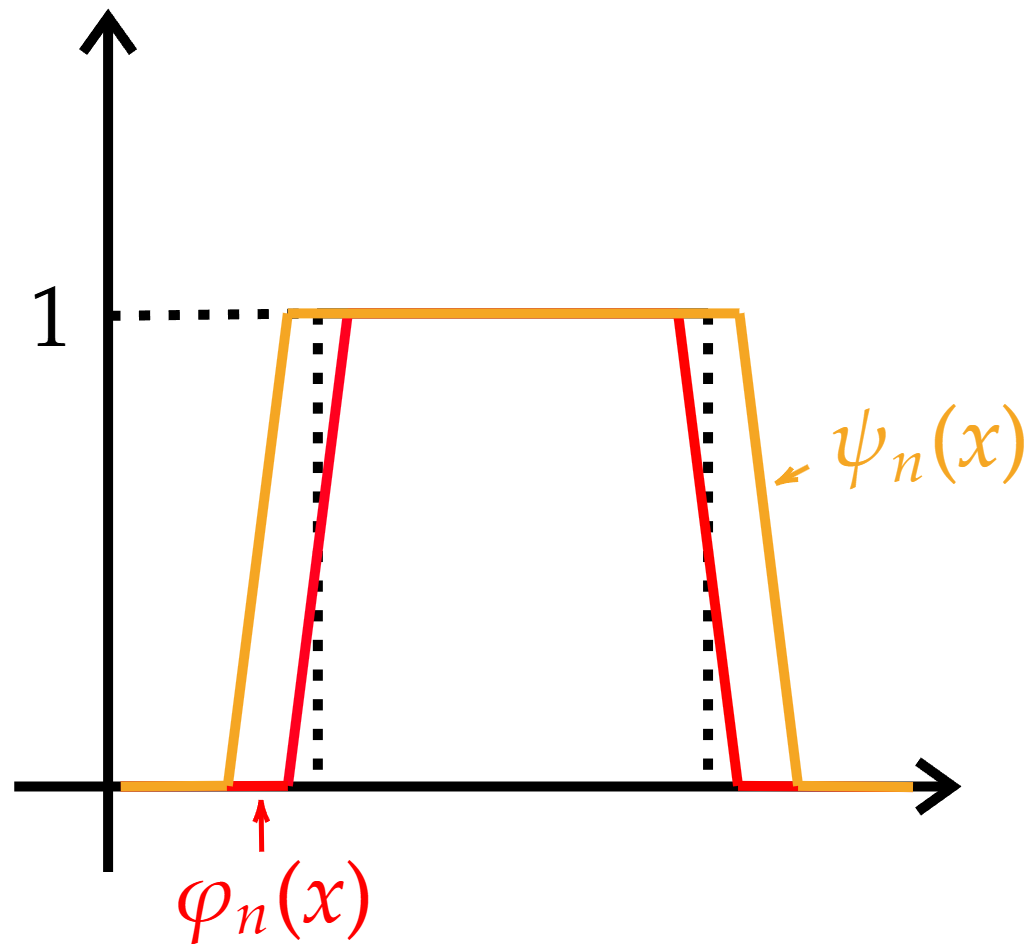
\includegraphics[width=1\textwidth]{fig/2.1.png}
    \end{minipage}\par
\end{proof}\par

\begin{itemize}
    \item 上述定理给了我们用连续函数刻画均匀分布的方法,如果我们把连续的条件加强为三阶连续可导,设$f \in C^3([0,1])$,$f(0)=f(1)$,由Fourier分析可知可以对上述函数作Fourier级数展开$f(x)=\frac{a_0}{2}+\sum_{n=1}^\infty(a_n\cos{2\pi nx}+b_n\sin{2\pi nx})\, (\forall\, x\in[0,1])$.并且有以下定理.
\end{itemize}

\begin{theorem*}
    $\frac{a_0}{2}+\sum_{n=1}^N(a_n\cos{2\pi nx}+b_n\sin{2\pi nx})\rightrightarrows f(x) \, (\forall\, x\in[0,1])$.
\end{theorem*}

借由Fourier级数,又可以得到以下使用正余弦和刻画均匀分布的方法.

\begin{theorem}
    $\forall\, f \in C^3([0,1]), f(0)=f(1),\frac{1}{N}\sum_{n=1}^N{f(x_n)}\to \int_{0}^{1}{f(x)}\d x$\par
    $\Leftrightarrow \frac{1}{N}\sum_{k=1}^N{\cos{2\pi kx_n}}\to 0,\frac{1}{N}\sum_{k=1}^N{\sin{2\pi kx_n}}\to 0$.\par
\end{theorem}
\begin{proof}
    \begin{itemize}
        \item[“$\Rightarrow$”] 取$f(x)=\cos{2\pi kx} \Rightarrow \frac{1}{N}\sum_{n=1}^N{\cos{2\pi kx_n}} \to \int_0^1{\cos{2\pi kx}} = 0$.\par
        对$\sin$的情形同理可证.
        \item[“$\Leftarrow$”] $\forall\, f \in C^3([0,1]),f(0)=f(1),\frac{a_0}{2}+\sum_{n=1}^N(a_n\cos{2\pi nx}+b_n\sin{2\pi nx})\rightrightarrows f(x)$\par
        $\Rightarrow \forall\, \varepsilon>0,\exists N,\text{s.t.}\left\lvert f(x) - \left(\frac{a_0}{2}+\sum_{n=1}^N(a_n\cos{2\pi nx}+b_n\sin{2\pi nx})\right)\right\rvert < \varepsilon,\,\forall\, x\in [0,1]$.\par
        记$\varphi_N(x) = \frac{a_0}{2}+\sum_{n=1}^N(a_n\cos{2\pi nx}+b_n\sin{2\pi nx})$\par
        则$\frac{1}{L}\sum_{i=1}^L{\varphi_N(x_n)} - \varepsilon \leq \frac{1}{L}\sum_{i=1}^L{f(x_n)} \leq \frac{1}{L}\sum_{i=1}^L{\varphi_N(x_n)} + \varepsilon$.\par
        令$L\to\infty$,则$\lim_{L\to\infty}\frac{1}{L}\sum_{i=1}^L{\varphi_N(x_n)}=\lim_{L\to\infty}{\frac{1}{L}\sum_{i=1}^L{\left(\frac{a_0}{2}+\sum_{n=1}^N(a_n\cos{2\pi nx}+b_n\sin{2\pi nx})\right)}}=\frac{a_0}{2}=\int_0^1{f(x)}\d x$.\par
        故上述不等式变为$\int_0^1{f(x)}\d x-\varepsilon \leq \varliminf_{n\to\infty}{\frac{1}{N}\sum_{n=1}^N{f(x_n)}} \leq \varlimsup_{n\to\infty}{\frac{1}{N}\sum_{n=1}^N{f(x_n)}} \leq \int_0^1{f(x)}\d x+\varepsilon$.\par
        再令$\varepsilon\to 0 \Rightarrow \frac{1}{N}\sum_{n=1}^N{f(x_n)}\to \int_{0}^{1}{f(x)}\d x$
    \end{itemize}
\end{proof}\par\noindent

\begin{itemize}
    \item 有了上述定理的准备,下一步要说明的是$\big\{\{n\log{2}\}\big\}_{n\in\mathbb{N}}$在$[0,1]$中均匀分布.\par
    \begin{proof}
        $\forall\, k \in \mathbb{N}$,考虑$\left| \frac{1}{N}\sum_{n=1}^{N-1}\cos \left(k\cdot\{n\log{2}\}2\pi\right) \right|$.\par
        由于添加整数对于$\cos \left(k\cdot\{n\log{2}\}2\pi\right)$的值没有影响,因此
        \begin{align*}
            \left| \frac{1}{N}\sum_{n=1}^{N-1}\cos \left(k\cdot\{n\log{2}\}2\pi\right) \right| &= \left| \frac{1}{N}\sum_{n=1}^{N-1}\cos \left(k\cdot n\log{2}\cdot 2\pi\right) \right| \\
            &= \left| \frac{1}{N}\sum_{n=0}^{N-1}{\frac{2\cos \left(k\cdot n\log{2}\cdot 2\pi\right)\sin \left(\log{2}\cdot k\pi\right)}{2\sin \left(\log{2}\cdot k\pi\right)}} \right| \\
            &\xlongequal{\text{积化和差}} \left|\frac{1}{N}\sum_{n=0}^{N-1}{\frac{\sin \left(\log{2}\cdot(2n+1)k\pi\right) - \sin \left(\log{2}\cdot(2n-1)k\pi\right)}{2\sin \left(\log{2}\cdot k\pi\right)}}\right| \\
            &= \left|\frac{1}{N}\frac{\sin \left(\log{2}\cdot(2N-1)k\pi\right) - \sin \left(\log{2}\cdot(-k\pi)\right)}{2\sin \left(\log{2}\cdot k\pi\right)}\right| \\
            &\leq \frac{1}{N}\frac{1}{\left|\sin \left(\log{2}\cdot k\pi\right)\right|} \to 0\,(N\to\infty)
        \end{align*}
        对$\sin$同理.
    \end{proof}
    \item $x_n=2^n,a_n=x_n\text{的首一数字}$,由于$\{n\log{2}\}$在$[0,1]$中均匀分布,因此\par
    $P(a_n=k)=\lim_{N\to\infty}{\frac{1}{N}\sum_{n=0}^N{\chi_{I_k}\big(\{n\log{2}\}\big)}} = \int_0^1{\chi_{I_k}(x)}\d x = \log{\left(1+\frac{1}{k}\right)} \, I_k=[\log{k},\log{(k+1)}]$.\par
    \item 这个结果就是大名鼎鼎的\bluebf{本$\cdot$福特定理}
\end{itemize}

在上面一系列的证明过程中,最重要的部分是对$\frac{1}{L}\sum_{n=1}^L{f(x)}$的估计,关于这个估计,我们先不加证明的引入以下定理:
\begin{theorem}{Birkhoff遍历定理}
    设$(X,\mathcal{B},m)$是一个概率测度空间,$T:(X,\mathcal{B},m)\to(X,\mathcal{B},m)$是一个保测遍历映射,那么$\forall\, f \in L^1(X,\mathcal{B},m)$,$\frac{1}{N}\sum_{n=0}^{N-1}{f(T^n(x))} \to \int_X{f}\d m\; \aew x$.
\end{theorem}
该定理包含的保测映射、遍历映射等概念将在后续学习中一一提及.

\section{保测映射}

\begin{definition}{保测映射}
    设$(X,\mathcal{B},m)$是一个概率测度空间,$T:(X,\mathcal{B}) \to (X,\mathcal{B})$是一个可测映射(可测集的原像是可测集).
    \begin{itemize}
        \item 如果$\forall\, A\in\mathcal{B}$,$m(T^{-1}A)=m(A)$,那么称$T$为保测映射.
        \item 如果$T$是$1-1$的保测映射且$T^-1$也是保测映射,那么称$T$为可逆保测映射
    \end{itemize}
\end{definition}
特别地,当映射$T:(X,\mathcal{B}) \to (X,\mathcal{B})$保持测度$m$不变时,我们就说$m$是$T$的\bluebf{不变测度},称$(X,\mathcal{B},m,T)$为\bluebf{概率系统}.\par
下面一个命题使用积分形式给出了保测映射的一个等价刻画.

\begin{proposition}{保测映射的等价刻画}
    $T:(X,\mathcal{B}) \to (X,\mathcal{B})$是一个保测映射$\Rightarrow \int_X{f\circ T}\d m=\int_X{f}\d m, \;\; \forall f\in L^1(X,\mathcal{B},m)$.
\end{proposition}
\begin{proof}
    先证明$\chi_B\circ T=\chi_{T^{-1}B}$.\par
    $\chi_B\circ T(x)=1,x\in X \Rightarrow T(x)\in B \Rightarrow x\in T^{-1}B \Rightarrow \chi_{T^{-1}B}(x)=1$. \par
    $\chi_B\circ T(x)=0,x\in X \Rightarrow T(x)\notin B \Rightarrow x\notin T^{-1}B \Rightarrow \chi_{T^{-1}B}=0$.\par
    所以$\chi_B\circ T=\chi_{T^{-1}B}$.\par
    \begin{itemize}[leftmargin=3.5em]
        \item[“$\Leftarrow$”] 令$f=\chi_B\;(B\in\mathcal{B})$.\par
        则$\int_X{\chi_B\circ T}\d m=\int_X{\chi_B}\d m \Leftrightarrow \int_X{\chi_{T^{-1}B}}\d m=\int_X{\chi_B}\d m \Leftrightarrow m(T^{-1}B)=m(B)$.\par
        \item[“$\Rightarrow$”] 假设$T$是保测映射,$\varphi(x)=\sum_{i=1}^n{c_i\chi_{A_i}(x)}$是简单函数.\par
        $\int_X{\varphi\circ T}\d m = \sum_{i=1}^n{c_i\int_X{\chi_{A_i}\circ T}\d m} = \sum_{i=1}^n{c_i\int_X{\chi_{T^{-1}A_i}}\d m} = \sum_{i=1}^n{c_i m(T^{-1}A_i)}$.\par
        $\int_X{\varphi}\d m=\sum_{i=1}^n{c_i\int_X{\chi_{A_i}}\d m} =\sum_{i=1}^n{c_i m(A_i)}$.\par
        由于$T$是保测映射,所以$m(T^{-1}A_i)=m(A_i)$,故$\int_X{\varphi\circ T}\d m=\int_X{\varphi}\d m$.\par
        对于$\forall f\in L^1(X,\mathcal{B},m),\, f\geq 0$,可找到一列简单函数$\varphi_n(x)\nearrow f(x)$,\par
        取极限得$\int_X{f\circ T}\d m=\int_X{f}\d m$.
    \end{itemize}
\end{proof}

除此之外,还有下述的帮助我们验证一个可测映射是否是保测映射的方法.

\begin{theorem}{保测映射的验证方法}
    设$(X,\mathcal{B},m)$是一个概率测度空间,$T:(X,\mathcal{B}) \to (X,\mathcal{B})$是一个可测映射.$\mathcal{S}$是$X$的一个生成$\mathcal{B}$的半代数,即$\mathcal{B}=\mathcal{B}(\mathcal{A}(\mathcal{S}))$,那么
    \[ T\text{是可测映射} \Longleftrightarrow \forall E \in \mathcal{S},m(T^{-1}E) = m(E) \]
\end{theorem}
\begin{proof}
    \begin{itemize}[leftmargin = 3.5em]
        \item[“$\Rightarrow$”] 由定义可得.
        \item[“$\Leftarrow$”] 令$\mathcal{F} = \{A\in\mathcal{B}|m(T^{-1}A)=m(A)\}$,下证$\mathcal{F}=\mathcal{B}(\mathcal{A}(\mathcal{S}))=\mathcal{B}$.\par
        \begin{enumerate}[(i)]
            \item $\mathcal{S}\subseteq\mathcal{F}$
            \item $\mathcal{A}(\mathcal{S})\subseteq\mathcal{F}$.\par
            $\forall E\in\mathcal{A}(\mathcal{S}),E=E_1\cup E_2\cup\cdots\cup E_n \;(E_1\in\mathcal{S},\,\text{两两不交})$.\par
            $\begin{aligned}
                m(T^{-1}E) &= m(T^{-1}E_1\cup T^{-1}E_2\cup\cdots\cup T^{-1}E_n)\\
                &=m(T^{-1}E_1)+m(T^{-1}E_2)+\cdots+m(T^{-1}E_n)\\
                &=m(E_1)+m(E_2)+\cdots+m(E_n)=m(E)
            \end{aligned}$\par
            \item $\mathcal{F}$是一个单调类.($\Rightarrow \mathcal{F}\supseteq\mathcal{C}(\mathcal{A}(\mathcal{S}))=\mathcal{B}(\mathcal{A}(\mathcal{S}))=\mathcal{B}$)\par
            设$A_1\subseteq A_2\subseteq \cdots\subseteq A_n\subseteq\cdots,\;A_i\in\mathcal{F}$.\par
            由于$T$是保测映射,所以$m(T^{-1}A_i)=m(A_i) \Leftrightarrow \int{\chi_{T^{-1}A_i}}\d m=\int {\chi_{A_i}}\d m$.\par
            由LDCT得$\int{\chi_{T^{-1}(\bigcup_{i=1}^\infty{A_i})}}\d m=\int{\chi_{(\bigcup_{i=1}^\infty{A_i})}}\d m \Leftrightarrow m\left(\bigcup_{i=1}^\infty{A_i}\right) = m\left(T^{-1}\left(\bigcup_{i=1}^\infty{A_i}\right)\right)$.\par
            $\Rightarrow \bigcup_{i=1}^\infty{A_i}\in\mathcal{F}$\par
            单调减的情形类似.
        \end{enumerate}
    \end{itemize}
\end{proof}
